\section{Introduction à l'étude}
\subsection{Sujet de l'étude}
L'objet de cette étude est d'évaluer différentes technologies permettant de mettre en place des connexions sécurisées via des Réseaux Privés Virtuels (VPN). L'objectif est de recenser plusieurs solutions fonctionnant sur divers systèmes d'exploitation et de les confronter entre-elles. Les différentes solutions seront d'abord évaluées en termes de complexité d'installation et d'administration, puis en termes de performances et de facilité d'utilisation.

VPN, ou Réseau Privé Virtuel, est le nom donné à une technologie permettant de relier des machines de façon sécurisée à travers un réseau non sûr comme Internet. Ce travail est effectué en vue de mettre en place une telle solution d'accès au sein de l'ISIMA. Les avantages d'une telle installation seraient multiples, du fait de la possibilité d'accéder au réseau interne de l'école depuis l'extérieur dans les mêmes conditions que si l'on était à l'intérieur.

Deux catégories de solutions VPN existent. On distingue les plate-formes dédiées tels les concentrateurs que les grands équipementiers proposent, et les solutions logicielles disponibles sur les systèmes d'exploitation courants : Microsoft a sa solution, le monde de l'Open-Source également.

Trois architecture ont donc été étudiées afin d'être en accord avec la diversité des solutions existantes : un routeur CISCO 2811XM configuré pour faire du VPN, un WindowsServer2K3 avec les services requis pour établir de connexions VPN, ainsi qu'un serveur Linux CentOS 5.1 avec le logiciel libre OpenVPN. La mise en place d'une plate-forme de test sera au coeur de cette étude.

% \subsection{Contexte de travail}
\subsection{Architecture étudiée}
\label{section_architecture_etudiee}
\subsubsection{Schéma logique}

Le travail a été intégralement réalisé dans la salle A214 de l'école. Nous avons pu mettre en place une maquette complète, permettant de simuler les accès depuis Internet vers un réseau interne. La figure \ref{schema-logique-maquette} présente un schéma logique de la maquette.

\begin{figure}[H]
	\begin{center}
% 		\includegraphics[width=\textwidth]{partie_1/images/schema_logique_maquette.JPG}\\
	\end{center}
	\caption{Schéma logique de la maquette}
	\label{schema-logique-maquette}
\end{figure}

\subsubsection{Schéma physique}

Pour faire cohabiter physiquement les trois architectures ensembles nous avons dû faire des conscessions. La plus importante a consisté à récupérer en DHCP les adresses IP des interfaces connectées au réseau de l'ISIMA, dans un coucis d'interropérabilité. La figure \ref{schema-physique-maquette} illustre l'architecture mise en place :

\begin{figure}[H]
	\begin{center}
	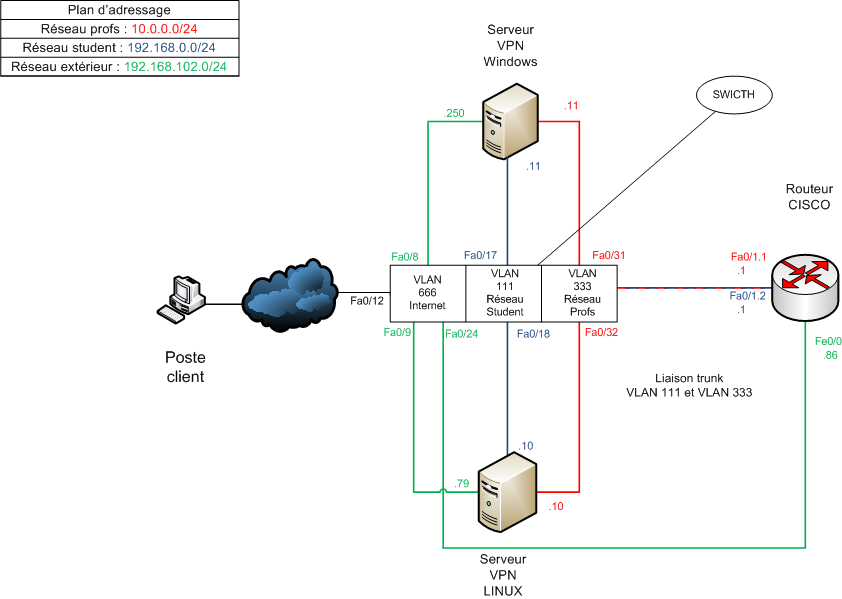
\includegraphics[width=\textwidth]{partie_1/images/archi_phy.png}\\
	\end{center}
	\caption{Schéma physique de la maquette}
	\label{schema-physique-maquette}
\end{figure}

\subsection{Etat de l'art}

\subsubsection{Le problème de la sécurité}

Comme expliqué précédemment, un VPN est une technologie permettant de créer des connexions sécurisés à travers un réseau non sûr. Il y a plusieurs menaces dont une connexion VPN doit être capable de nous protéger : l'espionnage, l'altération des données et le rejeu de paquets.

L'espionnage de données correspond à l'aspect le plus connu auquel sont confrontés les échanges, allant jusqu'à occulter (à tord) les deux autres. La parade contre l'espionnage consiste en la mise en place d'un chiffrement fort des données.

L'interception de données correspond au cas où un attaquant est présent en tant qu'intermédiaire dans le flot de communication, capable d'insérer, de modifier ou de supprimer des paquets circulant dans ce flot. Cette problématique a été à la fois la plus importante et la plus difficile à résoudre, la parade consistant à une authentification systématique en signant chaque paquet émis afin de pouvoir identifier ceux qui sont frauduleux. Le mécanisme le plus répendu d'authentification de paquet est nommé construction HMAC (Hash Message Authentication Code).

Le problème du rejeu est complémentaire de l'interception : il s'agit de réémettre des paquets valides ayant déjà circulé sur le réseau avec bien sûr de mauvaises intentions. La parade consiste ici à inclure un identifiant unique (ou un timestamp) pour chaque paquet dans sa signature. Lorsqu'une entité reçoit un paquet elle garde trace des identifiants unique déjà reçus et refuse un paquet qui serait déjà passé. Des implémentations d'algorithmes à glissement de fenêtre sont les protections les plus utilisées contre le rejeu.

\subsubsection{Le problème de l'authentification}

L'authentification des tiers est l'une des solutions clefs pour mettre en place des communications sécurisées. Néanmoins ce moyen de résoudre un problème ne fait que conduire à un autre plus gros encore : celui de la gestion des clefs. En effet les algorithmes utilisés pour le chiffrement des échanges réclament des clefs de session pour fonctionner, et pour que notre connexion puisse être considérée comme sécurisée ces clefs doivent changer régulièrement. Ainsi la mise en place d'une connexion sécurisée impose d'avoir un moyen d'échanger des clefs de session de façon sécurisée alors que notre connexion ne l'est pas encore : c'est la cryptographie à clefs privées qui va résout ce problème.



\subsubsection{Les différents types de VPN}

Il existe deux façons d'aborder la mise en place d'une technologie VPN, chacune ayant sa finalité : les VPN bridgés et les VPN routés. Les VPN bridgés sont généralement utilisés lors de connexions site-à-site, tandis que les VPN routés sont eux préférés pour connecter des clients nomades. La mise en place d'un VPN routé s'impose donc pour cette étude, car en plus d'être facilement intégrable à l'architecture existante, elle est parfaitement adaptée à l'usage que l'ISIMA pourrait en faire.

\subsubsection{Les classes de protocoles}
\paragraph{IPsec}
~

IPsec est une suite protocolaire de niveau 3, visant à apporter la sécurité manquant au protocole IP. Cette suite utilise plusieurs protocoles au cours des différentes phases de mise en place d'IPsec.

La première phase est une phase négociation au cours de laquelle les parties se mettent d'accord sur les algorithmes de chiffrement à utiliser et échangent des clefs de session via le protocole ISAKMP (Internet Security Association and Key Management Protocol). Au cours de cette phase le protocole IKE (Internet Key Exchange) intervient également pour générer ces clefs de session soit grâce à une clef partagée soit à l'aide de certificats RSA.

La seconde phase est la phase de communication au cours de laquelle les données peuvent traverser le tunnel et sont chiffrées. Deux protocoles peuvent intervenir en fonction de la finalité du tunnel : ESP qui fournit à la fois intégrité et confidentialité des données, et AH qui fournit l'intégrité et l'authentification.


\paragraph{pptp}
~

PPTP (Point to Point Tunneling Protocol) est un protocole dont le rôle consiste à construire des paquets PPP (Point to Point Protocole) pour les encapsuler dans des datagrammes IP. PPTP tire ainsi aventage des mécanismes d'authentification, de chiffrement et de compression déjà existants pour PPP (niveau 2) en les appliquant au niveau 3. Le principal aventage de ce protocole est son excellente intégration avec les systèmes Microsoft, au sein desquels la suite protocolaire de PPP a été réimplémentée pour accompagner PPTP.

Ainsi on utilise MS-Chap v2 (Microsoft-Challenge Handshake Authentication Protocol) pour l'authentification, et MPPe 'Microsoft Point to Point Encryption) pour le chiffrement. Au cours d'une session VPN entre un client et le serveur, une connexion TCP est utilisée pour le contrôle de la liaison. Quand à l'échange de données, celui-ci requiert un canal UDP et s'appuie sur le protocole GRE (Generic Routing Encapsulation).


\paragraph{TLS}
~

Le protocole TLS est une évolution du protocole SSL qui, après s'être rendu extrêmement populaire dans le domaine des transaction sécurisées au niveau applicatif (notamment le web), a être utilisé dans le domaine des VPN. Le but de ces technologies VPN est de s'appuyer sur la maturité de TLS pour gérer la gestion du tunnel de données ainsi que tous les éléments cryptographiques nécessaires : authentification, confidentialité et intégrité.

Une erreur commune est de penser que comme TLS n'est pas un protocole de niveau 3 les technologies s'appuyant sur lui ne répondent pas aux critères fondamentaux des VPN : il n'en est rien. Il s'agit simplement d'une approche différente du problème, issue d'une constatattion simple : Les systèmes complexes sont les plus difficiles à sécuriser. Là où la mise en place d'IPsec dépend d'une nouvelle pile IP et implique des intéractions à la fois très fortes et très sophistiquées avec le noyau du système, les technologies basées sur TLS s'appuient sur du code s'exécutant dans l'espace utilisateur : une simple interface réseau virtuelle est utilisée pour parvenir à ce résultat.


\subsection{Objectifs fixés}

Les objectifs de la suite de cette étude sont donc d'étudier la mise en place d'une plate-forme de test pour les différentes solutions qui ont été recensées conformément aux représentations logique et physique de l'architecture présentées en partie \ref{section_architecture_etudiee} page \pageref{section_architecture_etudiee}. Les différentes solutions seront finalement confrontées les uns aux autres dans une dernière partie.

Nous commencerons par étudier la solution Microsoft, viendra ensuite le logiciel OpenVPN sous Linux, et enfin la technologie CISCO. Pour la mise en place de chacune de ces trois solutions, nous nous attarderons sur les problématiques de l'installation et de la configuration, que ce soit côté serveur ou côté client. Chacune de ces parties fera état des problèmes rencontrés au cours de l'étude ainsi que des limites de chaque solution.

Les différentes solutions seront confrontées selon plusieurs critères prenant en compte les contraintes de sécurité des VPN. Elles seront d'abord évaluées en termes de complexité d'installation et d'administration, puis en termes de performances, de niveau de sécurité fourni et de facilité d'utilisation.

\pagebreak
